

\documentclass[accentcolor=tud4c,9.5pt,nochapname,bigchapter,paper=a5report]{tudreport}


\usepackage{mathtools}
\usepackage[pdftex,bookmarks=true]{hyperref}

\usepackage{lscape}
\usepackage{hyperref}
\usepackage{graphicx}
\usepackage{trfsigns}


\DeclareMathSizes{9.5}{9.5}{7}{7}
\DeclareMathSizes{10}{10}{7}{7}
\DeclareMathSizes{11}{11}{8}{8}

\usepackage{array}
\newcolumntype{+}{>{\global\let\currentrowstyle\relax}}
\newcolumntype{^}{>{\currentrowstyle}}
\newcommand{\rowstyle}[1]{\gdef\currentrowstyle{#1}%
#1\ignorespaces
}
\begin{document}

\def\Var{{\rm Var}\,}
\def\E{{\rm E}\,}
\def\freq{{\left(e^{j\omega}\right)}\,}


\title{Digital Signal Processing}
\subtitle{Formulary}
\subsubtitle{Author: Daniel Thiem - studium@daniel-thiem.de\\Version 0.1 - 10.02.2013}

\maketitle
\newpage
\thispagestyle{plain}
\mbox{}
\tableofcontents


\numberwithin{equation}{chapter}
\section*{Preface}
This formulary is based on the formulary of the course Stochastic Signals and Systems,
 which can be found here \url{https://github.com/Tyde/stosigsysfs/blob/master/document.pdf?raw=true}.
If you find any errors or have any ideas for improvement, mail me at studium@daniel-thiem.de
 or file an issue at \url{https://github.com/Tyde/dspformulary/issues}. The \LaTeX{}  source code is
online on \url{https://github.com/Tyde/dspformulary} and can be improved and extended.

\chapter{Digital Processing of Continous-Time Signals}
\section{Periodic Sampling}
Basic principles of sampling and transforming signals can be found in the Stochastic Signals and Systems formulary
\subsection{Reconstruction of Band-Limited Signals}
Assume, that $H_r(j\Omega)$ and $h_r(t)$ are the frequency and time responses for an ideal low pass filter where 
$x(n)$ is the input signal. Then the output will be
\begin{equation}
	x_r(t) = \sum\limits_{n=-\infty}^{\infty} x(n)h_r(t-nT)
\end{equation}
Because the filter is assumed to be ideal, its impulse response is given by:
\begin{equation}
	h_r(t)=\frac{\sin(\pi t/T)}{\pi t/T}
\end{equation}
where T is the sampling interval that should fulfil the Nyquist condition $\Omega_s > 2 \Omega_B$
\subsection{Discrete-time Processing of Continous-Time Signals}
To process a continous-time signal $x_c(t)$ with digital signal processing techniques, the following setup is used:\\
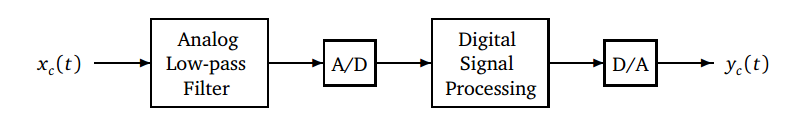
\includegraphics[width=\textwidth]{images/dsp_setup.png}

\chapter{Digital Filter Design}

Let $x(n)$ and $y(n) , n=0\pm 1,\ldots$ be the input and the output of the system.  
Linear time-invariant discrete-time systems can be characterized 
 by linear constant coefficient difference equations of the following type, where $\max(N-1,M)$ is the order:
 \begin {equation}
 \sum\limits_{k=0}^{M}a_ky(n-k)= \sum\limits_{r=0}^{N-1} b_r x(n-r)
 \end{equation}
\section{Finite Impulse Response (FIR) filter}
If $M=0$ then the impulse response of the filter is finite so that:
\begin{subequations}
\begin{align}
y(n) &= \frac{1}{a_0}\sum\limits_{k=-\infty}^{\infty}b_r x(n-k) \\
\text{comparison with } &\text{the convolution sum yields} \notag \\
h(n) &= \begin{cases}
b_n/a_n, &n=0,\ldots,N-1\\
0, &\text{otherwise}
\end{cases}
\end{align}
\end{subequations}

\section{Linear Phase Filters}
A digital filter can be described as linear phase filter if $H\freq$ can be expressed as:
\begin{equation}
	H\freq = H_M\freq e^{-j\omega \alpha}
\end{equation} 
with $H_M\freq$ real and $\alpha$(group delay) constant 

\subsection{Generalized linear phase system} \label{genLPS}
A Linear phase system with:
\begin{equation}
	H\freq = H_M\freq e^{-j\omega \alpha + j\beta}
\end{equation}
has to meet the condition:
\begin{equation} 
	\sum\limits_{n=-\infty}^{\infty} h(n)\sin[\omega (n-\alpha )+\beta] = 0 \forall \omega \in \mathbb{R}
\end{equation}

\section {Linear Phase FIR filters}
Applying the condition for generalized linear phase systems (\ref{genLPS}) to the FIR Filters yields two possible causal FIR Systems:
\begin{subequations}
\begin{align}
h(n) &= \begin{cases}
h(N-1-n)	&,0\leq n \leq N-1 \\
0			&,\text{otherwise} 
\end{cases} \\
H\freq &= H_e\freq e^{-j\omega (N-1)/2}
\end{align}
\end{subequations}
{\center and}
\begin{subequations}
\begin{align}
h(n) &= \begin{cases}
-h(N-1-n)	&,0\leq n \leq N-1 \\
0			&,\text{otherwise} 
\end{cases} \\
H\freq &= H_o\freq e^{-j\omega (N-1)/2+j\pi /2}
\end{align}
\end{subequations}

\section {Linear Phase FIR filter Types}
The linear phase FIR filters have been classified into 4 Types:

\begin{itemize}
  \item {\bf Type I} \quad symmetric impulse response and N is odd
  \item {\bf Type II}\quad symmetric impulse response and N is even
  \item {\bf Type III}\quad antisymmetric impulse response and N is odd
  \item {\bf Type IV}\quad antisymmetric impulse response and N is even
\end{itemize}

\subsection {Type I FIR linear phase filter}
$N$ is odd and the impuls response is symmetric. $\beta=0$ 
\begin{subequations}
\begin{align}
	h(n)&=h(N-1-n) \quad 0\leq n \leq N-1 \\
	H\freq &= e^{-j\omega \frac{N-1}{2}}\left[{\sum\limits_{k=0}^{(N-1)/2} a(k)\cos(\omega k)}\right]\\
	&\quad\text{where}\notag\\
	a(0)=h\left(\frac{N-1}{2}\right) \text{ and } a(k)&=2h\left(\frac{N-1}{2}-k\right), \quad\quad k=1,2,\ldots,(N-1)/2 \notag
\end{align}
\end{subequations}

\subsection {Type II FIR linear phase filter}
$N$ is even and the impuls response is symmetric. $\beta=0$ 
\begin{subequations}
\begin{align}
	h(n)&=h(N-1-n) \quad 0\leq n \leq N-1 \\
	H\freq &= e^{-j\omega \frac{N-1}{2}}\left\{{\sum\limits_{k=1}^{N/2} b(k)\cos\left[\omega \left(k-\frac{1}{2}\right)\right]}\right\}\\
	&\quad\text{where}\notag\\
	b(k)&=2h[N/2-k], \quad\quad k=1,2,\ldots,N/2 \notag
\end{align}
\end{subequations}

\subsection {Type III FIR linear phase filter}
$N$ is odd and the impuls response is antisymmetric. $\beta=\pi/2$ 
\begin{subequations}
\begin{align}
	h(n)&=-h(N-1-n) \quad 0\leq n \leq N-1 \\
	H\freq &= je^{-j\omega \frac{N-1}{2}}\left[{\sum\limits_{k=1}^{(N-1)/2} c(k)\sin(\omega k)}\right]\\
	&\quad\text{where}\notag\\
	c(k)&=2h[(N-1)/2-k], \quad\quad k=1,2,\ldots,(N-1)/2 \notag
\end{align}
\end{subequations}

\subsection {Type IV FIR linear phase filter}
$N$ is even and the impuls response is antisymmetric. $\beta=\pi/2$ 
\begin{subequations}
\begin{align}
	h(n)&=-h(N-1-n) \quad 0\leq n \leq N-1 \\
	H\freq &= je^{-j\omega \frac{N-1}{2}}\left\{{\sum\limits_{k=1}^{N/2} d(k)\sin\left[\omega \left(k-\frac{1}{2}\right)\right]}\right\}\\
	&\quad\text{where}\notag\\
	d(k)&=2h[N/2-k], \quad\quad k=1,2,\ldots,N/2 \notag
\end{align}
\end{subequations}

\section{FIR filter design}
\subsection{FIR filter type choice}
Not every FIR filter type fits on every filter. \\
\begin{tabular}{|+c|^c|^c|^c|^c|}
\hline
\rowstyle{\bfseries}

 Type & Low Pass & High Pass & Band Pass & Band Stop  \\ \hline
 I 	    & 			 &		      &			 & \\ \hline
 II 	& 			 &Not suitable&			 &Not suitable\\ \hline
 III 	&Not suitable&Not suitable&			 &Not suitable \\ \hline
 IV 	&Not suitable&		      &			 &Not suitable\\ \hline

\end{tabular}
\subsection{FIR filter design by Windowing}
Most idealized systems are non causal and have infinite impulse responses. To achieve finite impulse responses
and causality, truncating the ideal response is the most straightforward approach. \\
For the ideal impulse response 
\begin{equation}
h_d(n) = \frac{1}{2\pi}\int\limits_{-\pi}^{\pi} H_d\freq e^{j\omega n} d\omega
\end{equation}
the truncated response would be
\begin{subequations}
\begin{align}
h(n)&=\begin{cases}
h_d(n) &,0\leq n \leq N-1\\
0		&\text{, otherwise}
\end{cases} \\
\text{or}& \notag \\
h(n)&=h_d(n) \cdot w(n) \\
\text{with}& \notag \\
w(n) &= \begin{cases}
1 &,0\leq n \leq N-1\\
0		&\text{, otherwise}
\end{cases}\notag
\end{align}
\end{subequations}
\subsubsection{Properties of a rectangular Window}
If the window-funciton is a rectangle, the frequency response of the filter has to be multiplied with the 
fourier transform of the rectangle:
\begin{subequations}
\begin{align}
H\freq &= H_d\freq \circledast W\freq \\
&= H_d\freq \circledast \left[e^{-j\omega \frac{N-1}{2} } \cdot \frac{\sin(\omega N /2)}{\omega /2}\right]
\end{align}
\end{subequations}
This, if $H_d\freq$ should be closest to $H\freq$, $N$ has to go to infinity

\subsubsection{Main and Sidelobes}
With increasing $N$, the 'main-lobe' width increases. \\
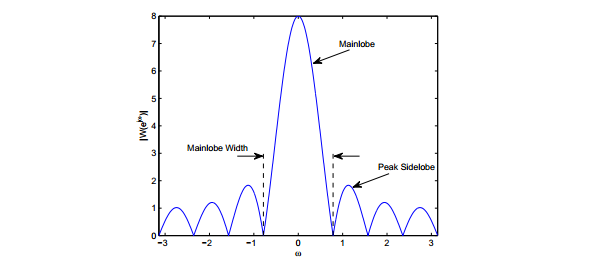
\includegraphics[width=\textwidth]{images/main_side_lobes.png}

\subsubsection{Peak approxomation error (PAE)}
\begin{equation}
 PAE =\gamma \cdot \max\limits_{\omega \in \mathbb{R}} \left|H_d\freq - H\freq\right|
\end{equation}
The PAE is also directly related to the maximum allowable specification tolerance.
With $\omega_c$ as the discontinuity of $H_d\freq$: 
\begin{equation}
\Delta H_d\left(e^{j\omega_c}\right) \cdot \gamma \leq \min(\alpha_1,\alpha_2)
\end{equation}

\subsubsection{Commonly used Windows}
\begin{subequations}
\begin{align}
\text{Rectangular} \notag \\
w(n) &= \begin{cases}
1 &,0\leq n \leq N-1\\
0		&\text{, otherwise}
\end{cases}\\
\text{Barlett} \notag \\
w(n) &= \begin{cases}
\frac{2n}{N-1} &,0\leq n \leq \frac{N-1}{2}\\
2-\frac{2n}{N-1}		&,\frac{N-1}{2}\leq n\leq N-1
\end{cases}\\
\text{Hanning} \notag \\
w(n)& = \frac{1}{2}\left[1-\cos\left(\frac{2\pi n}{N-1}\right)\right] \quad 0\leq n \leq N-1\\
\text{Hamming} \notag \\
w(n)& = 0.54-0.46\cos\left(\frac{2\pi n}{N-1}\right) \quad 0\leq n \leq N-1 \\
\text{Blackman} \notag \\
w(n)& = 0.42-0.5\cos\left(\frac{2\pi n}{N-1}\right)+0.08\cos\left(\frac{4\pi n}{N-1}\right) \quad 0\leq n \leq N-1
\end{align}
\end{subequations}
These windows have different Properties: \\
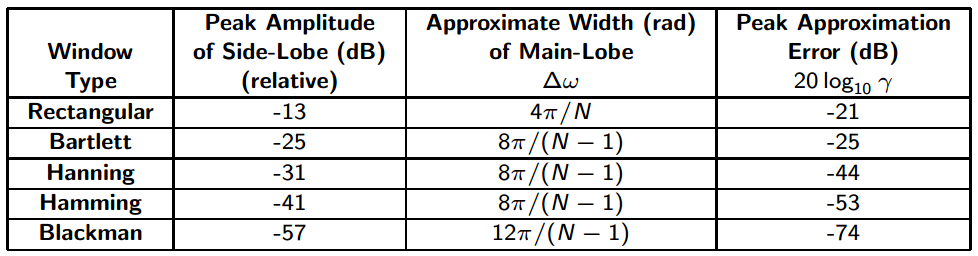
\includegraphics[width=\textwidth]{images/window_props.png}


\subsection{Kaiser Window Filter Design}
The Kaiser window function adapts to the specifications. Let $\alpha = \frac{N-1}{2}$ and $I_0$ be the zeroth
order modified Bessel function of the first kind:
\begin{equation}
w(n)=\begin{cases}
\frac{I_0\left\{\beta\left[1-\left(\frac{n-\alpha}{\alpha}\right)^2\right]^{\frac{1}{2}}\right\}}{I_0(\beta)} &,0\leq n\leq N-1\\
0 &,\text{otherwise}
\end{cases}
\end{equation}

\subsubsection{Desgin a filter with Kaiser window}
Assuming $\alpha_1 = \alpha_2$ and the transition region is $\Delta\omega = \omega_s-\omega_p$. With $A = -20\log_{10}\alpha_1$
\begin{equation}
\beta = \begin{cases}
0.1102(A-8.7) &A>50 \\
0.5842(A-21)^{0.4}+0.07866(A-21) &21\leq A \leq 50 \\
0 &A<21
\end{cases}
\end{equation}
and
\begin{equation}
N=\left[\frac{A-8}{2.285\Delta\omega}+1\right]
\end{equation}
\section{Infinite Impulse Response (IIR) filter}
IIR filters are systems, which follow the following Restrictions:\\
$h(n)$ is
  \begin{itemize}
  	\item real
  	\item causal
  	\item satifies stability
  \end{itemize}
$h(n)$ possesses a rational z-transform with $a_0=1$, i.e.
\begin{equation}
  	H(z)=\frac{\sum\limits_{k=0}^{N-1} b_k z^{-k}}{1-\sum\limits_{k=0}^{N-1} a_k z^{-k}}
  \end{equation}
  
 
\subsection{Properties of IIR filters}
\begin{itemize}
  \item {\bf Stability}\\ All poles of $H(z)$ must lie inside the unit disk
  \item {\bf Linear Phase}\\ IIR filters do not have linear phase. Only the magnitude response is specified.
\end{itemize}


\section {Filter Specficaion}
Non-ideal Filters have one or more pass-bands($\omega_p$), 
transition-bands(between $\omega_p$ and $\omega_s$) and stop-bands($\omega_s$). 
For the pass- and the stop- band, a tolerance
$\alpha_i$ has to be specified. Therefore a low-pass filter would have the following specification:
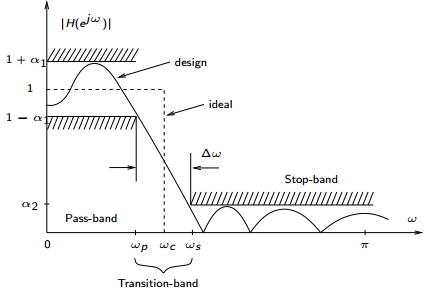
\includegraphics[width=\textwidth]{images/filter_spec.png}


\chapter{Miscellaneous}
\section{Useful mathematical equations}
\subsection{Geometric series}
\begin{equation}
\sum\limits_{n=0}^{N-1} q^n = \frac{1-q^N}{1-q} \quad \text{for} \quad|q|<1
\end{equation} 

\subsection{Conversion from Geometric series to trigonometric fraction}
Let $\frac{1-q^{N}}{1-q}$ be with $q = e^{-j\omega}$
\begin{equation}
\frac{1-e^{-jN\omega}}{1-e^{-j\omega}} = e^{-j\omega \frac{N-1}{2}}\frac{\sin\left(\frac{N}{2}\omega\right)}{\sin\left(\frac{\omega}{2}\right)}
\end{equation}
\end{document}
